\documentclass{Group_Templ}
\usepackage{eurosym}

\setlength{\parindent}{0pt}

\begin{document}

\section*{Exercise 4.2}
The half-space is defined as:
\[
	H=\{x\in \mathbb{R}^n | a^Tx\le b\}
\]


A set is convex if, for any two points $x,y \in H$,
every point on the line segment connecting them
also belongs to $H$.

Every point on this line segment can be expressed
as a convex combination:
\[
\lambda x + (1-\lambda)y,
\quad \lambda \in [0,1].
\]

Thus, to prove convexity, we must show that
\[
\lambda x + (1-\lambda)y \in H
\]
for all $x,y \in H$ and $\lambda \in [0,1]$.


Since $x,y\in H$, it follows that:

\[
	a^Tx\le b
\]
and
\[
	a^Ty\le b
\]

Since $\lambda \in [0,1]$, we have
$\lambda \geq 0$ and $1-\lambda \geq 0$.
Therefore, the convex combination satisfies:

\begin{flalign*}
	a^T(\lambda x+(1-\lambda)y) &= \lambda a^T x + (1-\lambda) a^T y \\
	&\le \lambda b + (1-\lambda) b \\
	&= b
\end{flalign*}


Thus, $\lambda x+(1-\lambda)y \in H$ for all
$x,y \in H$ and $\lambda \in [0,1]$.
Therefore, $H$ is convex by definition.
\section*{Exercise 4.3}
\begin{enumerate}
	\item 
\noindent\textbf{Given:}
\begin{align*}
	\text{Daily calorie requirement:} &\quad 1800\,\text{kcal}\\
	\text{Daily budget:} &\quad 11\,\text{\euro}\\
	\text{Mate:} &\quad 100\,\text{kcal},\ 1\,\text{\euro}\\
	\text{Pasta:} &\quad 300\,\text{kcal},\ 1\,\text{\euro}
\end{align*}

\begin{flalign*}
	x_1 = \text{Number of Mate},\quad &x_2 = \text{Number of Pasta} \\
	\max \quad x_1,\\
	\text{s.t.}\quad 100x_1+300x_2&\ge 1800, \\
	x_1+x_2&\le 11, \\
	x_1 &\ge 0, \\
	x_2 &\ge 0 \\
	\\
	\Leftrightarrow \\
	\max \quad x_1,\\
	\text{s.t.}\quad x_1&\ge18-3x_2, \\
	x_1&\le 11-x_2, \\
	x_1 &\ge 0, \\
	x_2 &\ge 0, \\
	\text{Objective function line: } x_1&=c \\
	c&=3 \Rightarrow x_1=3
\end{flalign*}
Please ignore the yellow marks on the left-hand side; they are remnants of erasing.\newline
\begin{minipage}[t]{\textwidth}
	\begin{figure}[H]
		\centering
		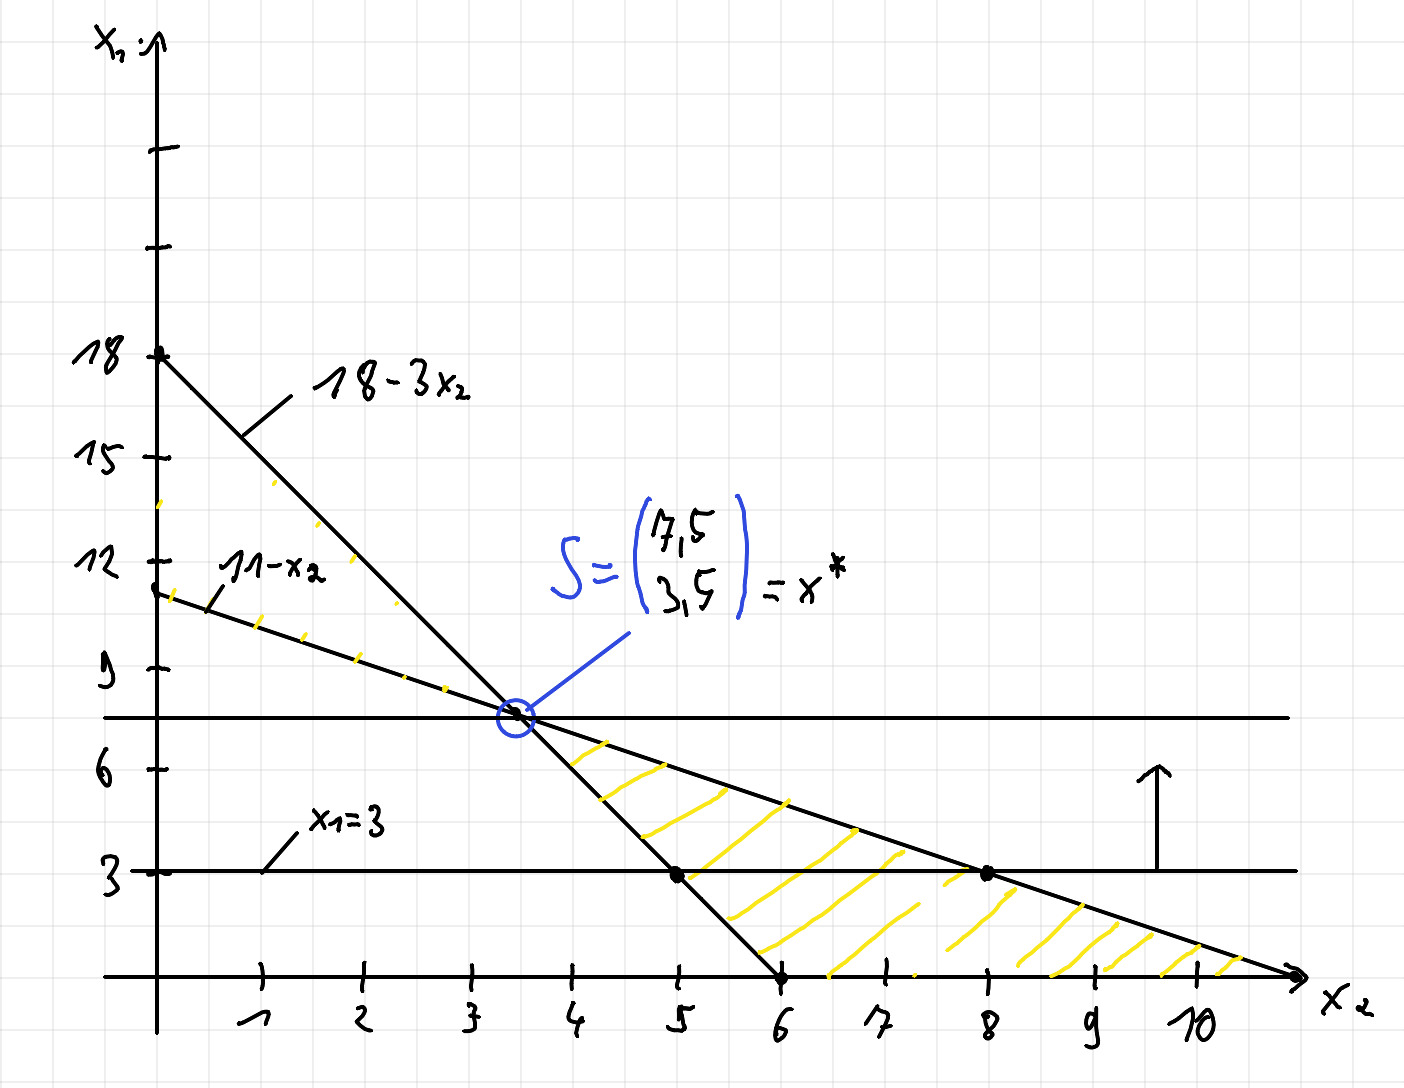
\includegraphics[width=0.8\textwidth]{4.3.1}
		\label{fig:label} % Optionales Label für Verweise
	\end{figure}
\end{minipage}


\noindent\textbf{Optimal solution:}

The optimal solution of the LP is
\[
x^* = (7.5, 3.5).
\]
Thus, we buy 7.5 bottles of mate and 3.5 packs
of pasta per day.

\noindent\textbf{Difference between LP and ILP:}

In an LP, variables may take real values, whereas
in an ILP, variables must take integer values.
Both must satisfy all constraints.

In this example, the optimal ILP solution is
\[
x^*_{\mathrm{ILP}} = (7,4).
\]
\item 
We assume a real-valued LP, as the exercise explicitly asks for a linear optimization problem rather than an ILP.

\textbf{Given:}
\begin{align*}
	\text{Maximum width:} &\quad 350\,\text{cm}\\
	\text{Mate width:} &\quad 6\,\text{cm}\\
	\text{Pasta width:} &\quad 4\,\text{cm}
\end{align*}
\begin{flalign*}
	x_1 = \text{Number of Mate},\quad &x_2 = \text{Number of Pasta}, d = \text{Number of days} \\
	\max \quad d,\\
	\text{s.t.}\quad 6x_1+4x_2&\le 350 \\
	x_1&\ge 7.5d, \\
	x_2&\ge 3.5d, \\
	x_1 &\ge 0, \\
	x_2 &\ge 0, \\
	d &\ge 0
\end{flalign*}
Deriving an upper bound for \(d\):

\begin{align*}
	350 &\geq 6x_1+4x_2\\
	&\geq 6(7.5d)+4(3.5d)\\
	&=59d
\end{align*}

Therefore,
\[
d\leq\frac{350}{59}.
\]

This upper bound is achieved by choosing
$x_1=7.5d$ and $x_2=3.5d$.

Resubstitute:
\begin{flalign*}
	x_1 &= 7.5d \\
	x_1 &= 7.5\cdot\frac{350}{59} \\
	x_1 &= \frac{2625}{59} \approx 44.4915 \\
	\\
	x_2 &= 3.5d \\
	x_2 &= 3.5\cdot\frac{350}{59} \\
	x_2 &= \frac{1225}{59} \approx 20.7627
\end{flalign*}
Therefore, the optimal solution is to buy approximately 44.49 bottles of mate and 20.76 packs of pasta, providing enough supplies for approximately 5.93 days.

However, since bottles and packs can only be purchased in whole units, this solution is a theoretical optimum and would not be directly feasible in practice.

\end{enumerate}

\end{document}
